\documentclass[a4paper]{article}

%=========================================
% Packages
%=========================================
\usepackage{mathtools}
\usepackage{amsfonts}
\usepackage{amsmath}
\usepackage{amssymb}
\usepackage{amsthm}
\usepackage[a4paper, total={6in, 8in}, margin=1in]{geometry}
\usepackage[utf8]{inputenc}
\usepackage{fancyhdr}
\usepackage[utf8]{inputenc}
\usepackage{graphicx}
\usepackage{physics}
\usepackage[listings]{tcolorbox}
\usepackage{hyperref}
\usepackage{tikz-cd}
\usepackage{adjustbox}
\usepackage{enumitem}
\usepackage[font=small,labelfont=bf]{caption}
\usepackage{subcaption}
\usepackage{wrapfig}
\usepackage{makecell}



\raggedright

\usetikzlibrary{arrows.meta}

\DeclarePairedDelimiter\ceil{\lceil}{\rceil}
\DeclarePairedDelimiter\floor{\lfloor}{\rfloor}

%=========================================
% Fonts
%=========================================
\usepackage{tgpagella}
\usepackage[T1]{fontenc}


%=========================================
% Custom Math Operators
%=========================================
\DeclareMathOperator{\adj}{adj}
\DeclareMathOperator{\im}{im}
\DeclareMathOperator{\nullity}{nullity}
\DeclareMathOperator{\sign}{sign}
\DeclareMathOperator{\dom}{dom}
\DeclareMathOperator{\lcm}{lcm}
\DeclareMathOperator{\ran}{ran}
\DeclareMathOperator{\ext}{Ext}
\DeclareMathOperator{\dist}{dist}
\DeclareMathOperator{\diam}{diam}
\DeclareMathOperator{\aut}{Aut}
\DeclareMathOperator{\inn}{Inn}
\DeclareMathOperator{\syl}{Syl}
\DeclareMathOperator{\edo}{End}
\DeclareMathOperator{\cov}{Cov}
\DeclareMathOperator{\vari}{Var}
\DeclareMathOperator{\cha}{char}
\DeclareMathOperator{\Span}{span}
\DeclareMathOperator{\ord}{ord}
\DeclareMathOperator{\res}{res}
\DeclareMathOperator{\Hom}{Hom}
\DeclareMathOperator{\Mor}{Mor}
\DeclareMathOperator{\coker}{coker}
\DeclareMathOperator{\Obj}{Obj}
\DeclareMathOperator{\id}{id}
\DeclareMathOperator{\GL}{GL}
\DeclareMathOperator*{\colim}{colim}

%=========================================
% Custom Commands (Shortcuts)
%=========================================
\newcommand{\CP}{\mathbb{CP}}
\newcommand{\GG}{\mathbb{G}}
\newcommand{\F}{\mathbb{F}}
\newcommand{\N}{\mathbb{N}}
\newcommand{\Q}{\mathbb{Q}}
\newcommand{\R}{\mathbb{R}}
\newcommand{\C}{\mathbb{C}}
\newcommand{\E}{\mathbb{E}}
\newcommand{\Prj}{\mathbb{P}}
\newcommand{\RP}{\mathbb{RP}}
\newcommand{\T}{\mathbb{T}}
\newcommand{\Z}{\mathbb{Z}}
\newcommand{\A}{\mathbb{A}}
\renewcommand{\H}{\mathbb{H}}
\newcommand{\K}{\mathbb{K}}

\newcommand{\mA}{\mathcal{A}}
\newcommand{\mB}{\mathcal{B}}
\newcommand{\mC}{\mathcal{C}}
\newcommand{\mD}{\mathcal{D}}
\newcommand{\mE}{\mathcal{E}}
\newcommand{\mF}{\mathcal{F}}
\newcommand{\mG}{\mathcal{G}}
\newcommand{\mH}{\mathcal{H}}
\newcommand{\mI}{\mathcal{I}}
\newcommand{\mJ}{\mathcal{J}}
\newcommand{\mK}{\mathcal{K}}
\newcommand{\mL}{\mathcal{L}}
\newcommand{\mM}{\mathcal{M}}
\newcommand{\mO}{\mathcal{O}}
\newcommand{\mP}{\mathcal{P}}
\newcommand{\mS}{\mathcal{S}}
\newcommand{\mT}{\mathcal{T}}
\newcommand{\mV}{\mathcal{V}}
\newcommand{\mW}{\mathcal{W}}

%=========================================
% Colours!!!
%=========================================
\definecolor{LightBlue}{HTML}{2D64A6}
\definecolor{ForestGreen}{HTML}{4BA150}
\definecolor{DarkBlue}{HTML}{000080}
\definecolor{LightPurple}{HTML}{cc99ff}
\definecolor{LightOrange}{HTML}{ffc34d}
\definecolor{Buff}{HTML}{DDAE7E}
\definecolor{Sunset}{HTML}{F2C57C}
\definecolor{Wenge}{HTML}{584B53}
\definecolor{Coolgray}{HTML}{9098CB}
\definecolor{Lavender}{HTML}{D6E3F8}
\definecolor{Glaucous}{HTML}{828BC4}
\definecolor{Mauve}{HTML}{C7A8F0}
\definecolor{Darkred}{HTML}{880808}
\definecolor{Beaver}{HTML}{9A8873}
\definecolor{UltraViolet}{HTML}{52489C}



%=========================================
% Theorem Environment
%=========================================
\tcbuselibrary{listings, theorems, breakable, skins}

\newtcbtheorem[number within = subsection]{thm}{Theorem}%
{	colback=Buff!3, 
	colframe=Buff, 
	fonttitle=\bfseries, 
	breakable, 
	enhanced jigsaw, 
	halign=left
}{thm}

\newtcbtheorem[number within=subsection, use counter from=thm]{defn}{Definition}%
{  colback=cyan!1,
    colframe=cyan!50!black,
	fonttitle=\bfseries, breakable, 
	enhanced jigsaw, 
	halign=left
}{defn}

\newtcbtheorem[number within=subsection, use counter from=thm]{axm}{Axiom}%
{	colback=red!5, 
	colframe=Darkred, 
	fonttitle=\bfseries, 
	breakable, 
	enhanced jigsaw, 
	halign=left
}{axm}

\newtcbtheorem[number within=subsection, use counter from=thm]{prp}{Proposition}%
{	colback=LightBlue!3, 
	colframe=Glaucous, 
	fonttitle=\bfseries, 
	breakable, 
	enhanced jigsaw, 
	halign=left
}{prp}

\newtcbtheorem[number within=subsection, use counter from=thm]{lmm}{Lemma}%
{	colback=LightBlue!3, 
	colframe=LightBlue!60, 
	fonttitle=\bfseries, 
	breakable, 
	enhanced jigsaw, 
	halign=left
}{lmm}

\newtcbtheorem[number within=subsection, use counter from=thm]{crl}{Corollary}%
{	colback=LightBlue!3, 
	colframe=LightBlue!60, 
	fonttitle=\bfseries, 
	breakable, 
	enhanced jigsaw, 
	halign=left
}{crl}

\newtcbtheorem[number within=subsection, use counter from=thm]{eg}{Example}%
{	colback=Beaver!5, 
	colframe=Beaver, 
	fonttitle=\bfseries, 
	breakable, 
	enhanced jigsaw, 
	halign=left
}{eg}

\newtcbtheorem[number within=subsection, use counter from=thm]{ex}{Exercise}%
{	colback=Beaver!5, 
	colframe=Beaver, 
	fonttitle=\bfseries, 
	breakable, 
	enhanced jigsaw, 
	halign=left
}{ex}

\newtcbtheorem[number within=subsection, use counter from=thm]{alg}{Algorithm}%
{	colback=UltraViolet!5, 
	colframe=UltraViolet, 
	fonttitle=\bfseries, 
	breakable, 
	enhanced jigsaw, 
	halign=left
}{alg}




%=========================================
% Hyperlinks
%=========================================
\hypersetup{
    colorlinks=true, %set true if you want colored links
    linktoc=all,     %set to all if you want both sections and subsections linked
    linkcolor=DarkBlue,  %choose some color if you want links to stand out
}


\pagestyle{fancy}
\fancyhf{}
\rhead{Labix}
\lhead{Algebraic Topology 3}
\rfoot{\thepage}

\title{Algebraic Topology 3}

\author{Labix}

\date{\today}
\begin{document}
\maketitle
\begin{abstract}
\begin{itemize}
\item Notes on Algebraic Topology by Oscar Randal-Williams
\end{itemize}
\end{abstract}
\pagebreak
\tableofcontents

\pagebreak

\section{Homotopy Theory}
\subsection{The nth Homotopy Groups}
\begin{defn}{Pairs of Space}{} Let $X$ be a topological space. A pair of space is a pair $(X,A)$ where $A\subseteq X$ is a subspace of $X$. A map of pairs $f:(X,A)\to(Y,B)$ is a continuous map $f:X\to Y$ such that $f(A)\subseteq B$. 
\end{defn}

\begin{defn}{Homotopy between Maps of Pairs}{} Let $f,g:(X,A)\to (Y,B)$ be maps of pairs. A homotopy between $f$ and $g$ is a homotopy $H:X\times[0,1]\to Y$ such that $H(A\times[0,1])\subseteq B$. 
\end{defn}

\begin{defn}{The nth Homotopy Groups}{} Let $(X,x_0)$ be a pointed space. Define the $n$th homotopy group $\pi_n(X,x_0)$ to be $$\pi_n(X,x_0)=\frac{\left\{\gamma:\left(I^n,\partial I^n\right)\to\left(X,\{x_0\}\right)\;\bigg{|}\;\gamma\text{ is continuous }\right\}}{\simeq}$$ where we say that $f\simeq g$ if there exists a homotopy between $f$ and $g$. 
\end{defn}

\begin{lmm}{}{} For any $n\in\N$, the two spaces $(I^n,\partial I^n)$ and $(S^n,s_0)$ are homotopy equivalent. 
\end{lmm}

\begin{defn}{Concatenation}{} For $n\geq 1$, define a composition law on $\pi_n(X,x_0)$ for a pointed space $(X,x_0)$ by the formula $$(f\cdot g)(t_1,\dots,t_n)=\begin{cases}
f(2t_1,t_2,\dots,t_n) & \text{ if } 0\leq t_1\leq\frac{1}{2}\\
g(2t_1-1,t_2,\dots,t_n) & \text{ if } \frac{1}{2}\leq t\leq 1
\end{cases}$$ for $f,g\in\pi_n(X,x_0)$. 
\end{defn}

\begin{thm}{}{} Let $(X,x_0)$ be a pointed space and $n\geq 1$. The operation $\cdot$ on $\pi_n(X,x_0)$ is well defined and endows it with the structure of a group. 
\end{thm}

\begin{prp}{}{} Let $(X,x_0)$ be a pointed space. Then $\pi_n(X,x_0)$ is abelian for $n\geq 2$. 
\end{prp}

An exercise in Hatcher shows that the coordinate chosen in the concatenation can be arbitrary, and will also result in an abelian group structure in $\pi_n(X,x_0)$. 

\subsection{Properties of Homotopy}
\begin{thm}{Functoriality}{} Let $(X,x_0)$ and $(Y,y_0)$ be pointed spaces and let $f:(X,x_0)\to(Y,y_0)$ be a pointed map. Then the induced map $$\pi_n(f):\pi_n(X,x_0)\to\pi_n(Y,y_0)$$ defined by $[\gamma]\mapsto[f\circ\gamma]$ is a group homomorphism. Moreover, it satisfies the following functorial properties. 
\begin{itemize}
\item If $g:(Y,y_0)\to(Z,z_0)$ is a pointed map then $$\pi_n(g\circ f)=\pi_n(g)\circ\pi_n(f)$$
\item If $\text{id}_{(X,x_0)}:(X,x_0)\to(X,x_0)$ is the identity map then $$\pi_n(\text{id}_{(X,x_0)})=\text{id}_{\pi_n(X,x_0)}$$
\end{itemize}
\end{thm}

Similar to all other functorial properties we have seen throughout algebraic topology, a homeomorphism of spaces give an isomorphism on homotopy groups. 

\begin{thm}{Homotopy Equivalence}{} Let $(X,x_0),(Y,y_0)$ be pointed spaces and $f,g:(X,x_0)\to (Y,y_0)$ be pointed maps. If $f$ and $g$ are homotopic, then the induced maps $$\pi_n(f)=\pi_n(g):\pi_n(X,x_0)\to\pi_n(Y,y_0)$$ are equal. Moreover, if $f$ is a homotopy equivalence, then $\pi_n(f)$ is an isomorphism. 
\end{thm}

\begin{prp}{}{} Let $(X,x_0)$ be a pointed space and let $p:(\tilde{X},\tilde{x}_0)\to(X,x_0)$ be a covering space. Then $p$ induces isomorphisms $$\pi_n(p):\pi_n(\tilde{X},\tilde{x}_0)\overset{\cong}{\longrightarrow}\pi_n(X,x_0)$$ for all $n\geq 2$. 
\end{prp}

\subsection{Relation to the Fundamental Group}
\begin{thm}{}{} Let $(X,x_0)$ and $(X,x_1)$ be pointed spaces with the same base space. Let $u:I\to X$ be a path from $x_0$ to $x_1$. Define the induced map $$u_\#:\pi_n(X,x_0)\to\pi_n(X,x_1)$$ as follows. For $[\gamma]\in\pi_n(X,x_0)$ define $u_\#([\gamma])$ by first shrinking the domain of $\gamma$ to a smaller concentric cube in $I^n$. Then inserting the path $\gamma$ on each radical segment of the shell between the smaller cube and $\partial I^n$. \\~\\
The construction of $u_\#$ is a group isomorphism. Moreover, it satisfies the following universal properties. 
\begin{itemize}
\item If $v:I\to X$ is a path from $x_1$ to $x_2$ and $u\cdot v$ is the concatenation of these paths, then $$(u\cdot v)_\#=u_\#\circ v_\#$$
\item If $c_{x_0}$ is the constant path from $x_0$ to $x_0$ then $(c_{x_0})_\#$ is the identity
\end{itemize}
\end{thm}

\begin{prp}{}{} Let $(X,x_0)$ and $(X,x_1)$ be pointed spaces with the same base space. Let $u,v:I\to X$ be paths from $x_0$ to $x_1$. If $u$ and $v$ are homotopic relative to end points then the induced maps $$u_\#=v_\#:\pi_n(X,x_0)\to\pi_n(X,x_1)$$ are equal. 
\end{prp}

\begin{crl}{}{} Let $(X,x_0)$ and $(X,x_1)$ be pointed spaces with the same base space. If $x_0$ and $x_1$ are path connected, then $$\pi_n(X,x_0)\cong\pi_n(X,x_1)$$ where the isomorphism depends on the choice of path from $x_0$ to $x_1$. 
\end{crl}

This also shows that if $X$ is path connected, then $\pi_n(X,x_0)$ no longer depends on the choice of base point. Although there are no canonical isomorphisms between $\pi_n(X,x_0)$ and $\pi_n(X,x_1)$, we still forget about the base point in this case and write the homotopy groups as $\pi_n(X)$. 

\begin{prp}{}{} Let $(X,x_0)$ be a pointed space and $f\in\pi_n(X,x_0)$. Let $u:I\to X$ be a loop on $x_0$. Then $u$ induces a left action of $\pi_1(X,x_0)$ on $\pi_n(X,x_0)$ by the map $$(u,\gamma)\mapsto\left(u_\#(\gamma)\right)$$ In particular, for $n\geq 2$, $\pi_n(X,x_0)$ is a $\Z\pi_1(X,x_0)$-module. 
\end{prp}

\begin{prp}{}{} Let $X_i$ for $i\in I$ be a family of path connected spaces. Then there are isomorphisms $$\pi_n\left(\prod_{i\in I}\right)\cong\prod_{i\in I}\pi_n(X_i)$$
\end{prp}

\subsection{Relative Homotopy Groups}
\begin{defn}{Triplets of Spaces}{} Let $X$ be a topological space. A pointed pair of space is a triple $(X,A_1,A_2)$ where $A_2\subseteq A_1\subseteq X$ are subspaces of $X$. A map between triplets of spaces $f:(X,A_1,A_2)\to(Y,B_1,B_2)$ is a map $f:X\to Y$ such that $f(A_1)\subseteq B_1$ and $f(A_2)\subseteq B_2$. \\~\\
If $A_2=\{x_0\}$ is a single point we say that $(X,A,x_0)$ is a pointed pair of spaces. 
\end{defn}

\begin{defn}{Homotopy between Maps of Triplets}{} Let $f,g:(X,A_1,A_2)\to(Y,B_1,B_2)$ be maps triplets of spaces. A homotopy between $f$ and $g$ is a homotopy between $f:X\to Y$ and $g:X\to Y$, namely $H:X\times[0,1]\to Y$ such that $H(A_1\times[0,1])\subseteq B_1$ and $H(A_2\times[0,1])\subseteq B_2$. 
\end{defn}

\begin{defn}{The nth Relative Homotopy Groups}{} Let $(X,A,x_0)$ be a pointed pair of space. Let $n\geq 2$. Regard $I^{n-1}$ sitting inside $I^n$ by $I^{n-1}=\{(x_1,\dots,x_n)\in I^n\;|\;x_n=0\}$ and let $J^{n-1}=\overline{\partial I^n\setminus I^{n-1}}$. Define the relative homotopy groups of the triple by $$\pi_n(X,A,x_0)=\frac{\left\{\gamma:\left(I^n,\partial I^n,J^{n-1}\right)\to\left(X,A,x_0\right)\;\bigg{|}\;\gamma\text{ is continuous }\right\}}{\simeq}$$ where we say that $f\simeq g$ if there exists a homotopy between $f$ and $g$. 
\end{defn}

It is easy to see that $\pi_n(X,x_0,x_0)=\pi_n(X,x_0)$ so that homotopy groups are a special case of the relative homotopy groups. 

\begin{lmm}{}{} For any $n\in\N$, the two triplets $(I^n,\partial I^n,J^{n-1})$ and $(D^n,S^{n-1},s_0)$ are homotopy equivalent. 
\end{lmm}

\begin{thm}{}{} Let $(X,A,x_0)$ be a pointed pair of space. The composition law on definition 1.1.4 defines a group structure on $\pi_n(X,A,x_0)$ for $n\geq 2$. Moreover, $\pi_n(X,A,x_0)$ is abelian for $n\geq 3$. 
\end{thm}

\subsection{Induced Maps of Relative Homotopy Groups}
\begin{thm}{}{} Let $(X,A,x_0)$ and $(Y,B,y_0)$ be pointed pairs of spaces and $f:(X,A,x_0)\to(Y,B,y_0)$ a map. Then $f$ induces a map on the relative homotopy groups $$f_\ast:\pi_n(X,A,x_0)\to\pi_n(Y,B,y_0)$$ for $n\geq 2$ satisfying the following functorial properties: 
\begin{itemize}
\item $f_\ast$ is a group homomorphism
\item If $g:(Y,B,y_0)\to(Z,C,z_0)$ is a map, then $$(g\circ f)_\ast=g_\ast\circ f_\ast$$
\item If $\text{id}_{(X,A,x_0)}$ is the identity map on $(X,A,x_0)$, then $$(\text{id}_{(X,A,x_0)})_\ast=\text{id}_{\pi_n(X,A,x_0)}$$
\end{itemize}
\end{thm}

\begin{prp}{}{} Let $(X,A,x_0),(Y,B,y_0)$ be pointed pairs of spaces and $f,g:(X,A,x_0)\to (Y,B,y_0)$ be pointed maps. If $f$ and $g$ are homotopic, then the induced maps $$f_\ast=g_\ast:\pi_n(X,A,x_0)\to\pi_n(Y,B,y_0)$$ are equal. Moreover, if $f$ is a homotopy equivalence, then $f_\ast$ is an isomorphism. 
\end{prp}

TBA: change of base point isomorphisms. 

\begin{thm}{The Hurewicz Homomorphism}{} Let $(X,A,x_0)$ be a pointed pair of space. Let $u_n$ be a generator of $H_n(S^n)\cong\Z$. Then the map $$h:\pi_n(X,A,x_0)\to H_n(X,A)$$ defined by $[f]\mapsto f_\ast(u_n)$ is a group homomorphism. 
\end{thm}

\subsection{Long Exact Sequence in Homotopy Groups}
\begin{thm}{}{} Let $X$ be a space and $A,B$ be subspaces of $X$ such that $B\subseteq A\subseteq X$. Let $x_0\in B$. Then there is a long exact sequence in relative homotopy groups: \\~\\
\adjustbox{scale=0.88,center}{\begin{tikzcd}
	\cdots & {\pi_n(A,B,x_0)} & {\pi_n(X,B,x_0)} & {\pi_n(X,A,x_0)} & {\pi_{n-1}(A,B,x_0)} & \cdots & {\pi_1(X,A,x_0)}
	\arrow[from=1-1, to=1-2]
	\arrow["{i_\ast}", from=1-2, to=1-3]
	\arrow["{j_\ast}", from=1-3, to=1-4]
	\arrow["{\partial_n}", from=1-4, to=1-5]
	\arrow[from=1-5, to=1-6]
	\arrow[from=1-6, to=1-7]
\end{tikzcd}}\\~\\
where $i:(A,B,x_0)\to(X,B,x_0)$ and $j:(X,B,x_0)\to(X,A,x_0)$ are the inclusions and $\partial:\pi_n(X,A,x_0)\to\pi_{n-1}(A,B,x_0)$ is given by $[\gamma]\mapsto[\gamma|_{I^{n-1}}]$
\end{thm}

TBA: Naturality of the sequence. 

\begin{thm}{}{} Let $(X,A,x_0)$ be a pointed pair of spaces. The relative homotopy groups and (absolute) homotopy groups of $(X,A,x_0)$ fit into a long exact sequence \\~\\
\adjustbox{scale=0.75,center}{\begin{tikzcd}
	\cdots & {\pi_{n+1}(X,A,x_0)} & {\pi_n(A,x_0)} & {\pi_n(X,x_0)} & {\pi_n(X,A,x_0)} & {\pi_{n-1}(A,x_0)} & \cdots & {\pi_0(X,x_0)} & 0
	\arrow[from=1-1, to=1-2]
	\arrow["{\partial_{n+1}}", from=1-2, to=1-3]
	\arrow["{i_\ast}", from=1-3, to=1-4]
	\arrow["{j_\ast}", from=1-4, to=1-5]
	\arrow["{\partial_n}", from=1-5, to=1-6]
	\arrow[from=1-6, to=1-7]
	\arrow[from=1-8, to=1-9]
	\arrow[from=1-7, to=1-8]
\end{tikzcd}}\\~\\
where $\partial_n$ is defined by $[f]\mapsto [f|_{I^{n-1}}]$ and $i_\ast$ and $j_\ast$ are induced by inclusions. 
\end{thm}

Note that even though at the end of the sequence group structures are not defined, exactness still makes sense: kernels in this case consists of elements that map to the homotopy class of the constant map. 


\subsection{n-Connectedness}
\begin{defn}{n-Connected Space}{} Let $X$ be a space. We say that it is $n$-connected if $$\pi_k(X,x_0)=0$$ for $0\leq k\leq n$ and some $x_0\in X$. 
\end{defn}

Note that $\pi_0(X,x_0)$ implies that $X$ is path connected. Hence the notion of $n$-connectedness does not depend on the base point by the change of base point isomorphism. In particular, $\pi_k(X,x_0)=0$ for $0\leq k\leq n$ and some $x_0\in X$ if and only if $\pi_k(X,x_0)=0$ for $0\leq k\leq n$ for all $x_0\in X$. (Hatcher)

\begin{defn}{n-Connected Pair of Spaces}{} Let $(X,A)$ be a pair of space. We say that it is $n$-connected if $$\pi_k(X,A,x_0)=0$$ for $0\leq k\leq n$ and all $x_0\in A$. 
\end{defn}

TBA: conditions in P.346 of Hatcher

\begin{defn}{Weakly Contractible}{} Let $X$ be a space. We say that $X$ is weakly contractible if $$\pi_n(X)=0$$ for all $n\geq 0$. 
\end{defn}

\pagebreak
\section{Homotopy and CW-Complexes}
\subsection{Weak Homotopy Equivalence}
\begin{defn}{Weak Homotopy Equivalence}{} We say that a map $f:X\to Y$ is a weak homotopy equivalence if it induces isomorphisms on all homotopy groups $\pi_n$ on any choice of base point. 
\end{defn}

TBA: compression lemma in Hatcher

\begin{thm}{}{} Let $X,Y$ be spaces and let $f:X\to Y$ be a weak homotopy equivalence. Then $f$ induces isomorphisms $$f_\ast:H_n(X;G)\overset{\cong}{\longrightarrow}H_n(Y;G)\;\;\;\;\text{ and }\;\;\;\;f^\ast:H^n(Y;G)\overset{\cong}{\longrightarrow}H^n(X;G)$$ for any group $G$ and all $n\in\N$. 
\end{thm}

\begin{prp}{}{} Let $X,Y$ be spaces and let $f:X\to Y$ be a weak homotopy equivalence. Then $f$ induces bijections $$[Z,X]\cong[Z,Y]\;\;\;\;\text{ and }\;\;\;\;[Z,X]_\ast\cong[Z,Y]_\ast$$ for all $CW$-complexes $Z$. 
\end{prp}

\subsection{Whitehead's Theorem}
\begin{thm}{Whitehead's Theorem}{} If $X$ and $Y$ are CW-complexes and $f:X\to Y$ is a weak homotopy equivalence, then $f$ is a homotopy equivalence. 
\end{thm}

TBA: extension lemma in Hatcher. 

\begin{crl}{}{} If $X$ and $Y$ are CW-complexes with $\pi_1(X)=\pi_1(Y)=0$ and $f:X\to Y$ induces isomorphisms on homology groups $H_n$ for all $n$, then $f$ is a homotopy equivalence. 
\end{crl}

\subsection{Cellular Approximations}
\begin{defn}{Cellular Maps}{} Let $X$ and $Y$ be CW-complexes. A map $f:X\to Y$ is called cellular if $f(X_n)\subset Y_n$ for all $n$, where $X_n$ is the $n$-skeleton of $X$. 
\end{defn}

\begin{defn}{Cellular Approximations}{} Let $X$ and $Y$ be CW-complexes. We say that $f:X\to Y$ has a cellular approximations if $f$ is homotopic to a cellular map $f':X\to Y$. 
\end{defn}

\begin{thm}{Cellular Approximation Theorem}{} Any map $f:X\to Y$ between CW-complexes has a cellular approximation $f':X\to Y$. Moreover, if $f$ is already cellular on a subcomplex $A\subseteq X$, then we can take $f'|_A=f|_A$. 
\end{thm}

\begin{thm}{Relative Cellular Approximation}{} Any map $f:(X,A)\to (Y,B)$ between pairs of CW-complexes has a cellular approximation. 
\end{thm}

\begin{crl}{}{} Let $A\subset X$ be CW-complexes and suppose that all cells $X\setminus A$ have dimension larger than $n$. Then $(X,A)$ is $n$-connected. 
\end{crl}

\begin{crl}{}{} Let $X$ be a CW complex and let $X^n$ be its $n$-skeleton. Then $(X,X^n)$ is $n$-connected. Moreover, the inclusion $X^n\hookrightarrow X$ induces an isomorphism $$\pi_k(X^n)\to\pi_k(X)$$ for $0\leq k<n$ and a surjection for $k=n$. 
\end{crl}

\subsection{CW Approximations}
\begin{defn}{CW Approximation}{} Let $X$ be a space. A CW approximation of $X$ is a weak homotopy equivalence $f:Z\to X$ where $Z$ is a CW complex. 
\end{defn}

The goal of this section is that every space has a CW approximation. The given homotopy equivalence makes this notion powerful because this means that for any space $X$, there exists a CW-complex such that $X$ and $Z$ are homotopy equivalent, and moreover, has isomorphic homotopy, homology and cohomology groups. 

\begin{defn}{CW Model}{} Let $(X,A)$ be a non-empty pair of CW-complexes. An $n$-connected CW model of $(X,A)$ is an $n$-connected CW pair $(Z,A)$ together with a map $f:Z\to X$ with $f|_A=\text{id}_A$ such that $$f_\ast:\pi_i(Z)\to\pi_i(X)$$ is an isomorphism for $i>n$ and an injection for $i=n$ for any choice of base point. 
\end{defn}

\begin{thm}{}{} For any non-empty pair $(X,A)$ of CW-complexes, there exists an $n$-connected model $(Z,A)$. Moreover, $Z$ can be built from $A$ by attaching cells of dimension greater than $n$. 
\end{thm}

\begin{crl}{}{} Every pair of CW-complex $(X,A)$ has a CW approximation $(Z,B)$. 
\end{crl}

Thus we have shown existence of CW approximations, it remains to show uniqueness. 

\begin{crl}{}{} CW-approximations are unique up to homotopy equivalence. 
\end{crl}

\pagebreak

\section{Main Results of Homotopy Theory on CW-Complexes}
\subsection{Excision for Homotopy Groups}
\begin{thm}{The Homotopy Excision Theorem}{} Let $X$ be a CW-complex and $A,B$ be sub complexes such that $X=A\cup B$ and $A\cap B\neq\emptyset$. If $(A,A\cap B)$ is $m$-connected and $(B,A\cap B)$ is $n$-connected for $m,n\geq 0$, then the map $$\iota_\ast:\pi_i(A,A\cap B)\to(X,B)$$ induced by the inclusion $\iota:(A,A\cap B)\to(X,B)$ is an isomorphism for $0\leq i<m+n$ and a surjection for $i=m+n$. 
\end{thm}

\begin{prp}{}{} Let $(X,A)$ be a pair of $r$-connected CW complexes and let $A$ be $s$-connected. Then the map $$p_\ast:\pi_k(X,A)\to\pi_k(X/A)$$ induced by the quotient map $p:X\to X/A$ is an isomorphism for $0\leq k\leq r+s$ and a surjection for $k=r+s+1$. 
\end{prp}

\subsection{Freudenthal Suspension Theorem}
\begin{defn}{Reduced Suspension}{} Let $(X,x_0)$ be a pointed space. Define the reduced suspension of $X$ to be the space $$\Sigma X=\frac{X\times I}{(X\times\{0\}\cup X\times\{1\}\cup\{x_0\}\times I)}$$
\end{defn}

The reduced suspension defines a continuous map sending a space $X$ to its reduced suspension $\Sigma X$. 

\begin{thm}{Freudenthal Suspension Theorem}{} Let $X$ be an $n$-connected CW complex. Then for $0\leq k\leq 2n$, the induced map $$\Sigma_\ast:\pi_k(X)\to\pi_{k+1}(\Sigma X)$$ is an isomorphism. For $k=2n+1$, $\Sigma_\ast$ is a surjection. 
\end{thm}

We can keep on suspending the space and the maps. Indeed if $X$ is $n$-connected then, by Freudenthal suspension theorem $\Sigma X$ is $(n+1)$-connected. We can then apply the suspension theorem again on $\Sigma X$ and we see that $\Sigma^2X$ is $(n+2)$-connected. 

\begin{crl}{}{} There is an isomorphism $$\pi_{n+k}(S^n)\cong\pi_{n+k+1}(S^{n+1})$$ for all $n\geq k+2$. 
\end{crl}

\begin{defn}{Stable Homotopy Groups}{} Let $X$ be a space. Let $n\in\N$. Define the $n$th stable homotopy groups of $X$ to be $$\pi_n^s(X)=\colim_{k\to\infty}\pi_{n+k}(\Sigma^kX)$$
\end{defn}

\begin{prp}{}{} Let $X$ be a space. Let $k\in\N$. Then the the following sequence of suspensions $$\pi_k(X)\to\pi_{k+1}(\Sigma X)\to\pi_{k+2}(\Sigma^2X)\to\cdots$$ are eventually isomorphisms. \tcbline
\begin{proof}
Let $X$ be $n$-connected. There are two cases. \\~\\

Let $k\leq 2n$. By Freudenthal suspension theorem, if $k\leq 2n$ then $\pi_k(X)\cong\pi_{k+1}(\Sigma X)$. Then $\Sigma X$ is $(n+1)$-connected hence $\pi_{k+1}(\Sigma X)\cong\pi_{k+2}(\Sigma^2X)$ is an isomorphism since $k+1\leq 2n+2$. More generally, for $r\in\N$, $\Sigma^rX$ is $(r+n)$-connected hence $$\pi_{k+r}(\Sigma^rX)\cong\pi_{k+r+1}(\Sigma^{r+1}X)$$ is an isomorphism since $k+r\leq 2n+2r$. \\~\\

Now if $k>2n$, then there exists $r\in\N$ such that $k+r\leq 2n+2r$. Such an $r$ is given by say $k-2n$. Then by Freudenthal suspension theorem, $$\pi_{k+r}(\Sigma^rX)\cong\pi_{k+r+1}(\Sigma^{r+1}X)$$ is an isomorphism. More generally, for $m\in\N$, $\Sigma^{r+m}X$ is $(r+m+n)$-connected hence $$\pi_{k+r+m}(\Sigma^{r+m}X)\cong\pi_{k+r+m+1}(\Sigma^{r+m+1}X)$$ is an isomorphism since $k+r+m\leq 2n+2r+2m$. 
\end{proof}
\end{prp}

\subsection{Hurewicz's Theorem}
\begin{thm}{Hurewicz's Homomorphism}{} Let $X$ be a path connected space. Then for any $n\in\N$, there is a group homomorphism $$h_n:\pi_n(X)\to H_n(X)$$ called the Hurewicz homomorphism, defined as follows. Let $[u_n]\in H_n(S^n)$ be a canonical generator. Then $h_n([f])=f_\ast(u_n)$. 
\end{thm}

\begin{thm}{Hurewicz's Theorem}{} Let $X$ be a space. Then the following are true regarding Hurewicz's homomorphism. 
\begin{itemize}
\item Let $n\geq 2$. If $X$ is $(n-1)$-connected, then $\widetilde{H}_k(X)=0$ for all $0\leq k<n$. Moreover, the Hurewicz homomorphism $$h_n:\pi_n(X)\to H_n(X)$$ is an isomorphism. Moreover, $h_{n+1}$ is a surjection. 
\item Let $n=1$, then Hurewicz's homomorphism induces an isomorphism $$\overline{h_1}:\pi_1(X)^\text{ab}\to H_1(X)$$ 
\end{itemize}
\end{thm}

\begin{thm}{Relative Hurewicz's Homomorphism}{} Let $(X,A)$ be a pair of spaces. Then for any $n\geq 1$, there is a group homomorphism $$h_n:\pi_n(X,A)\to H_n(X,A)$$ called the relative Hurewicz homomorphism, defined as follows. Let $[u_n]\in H_n(S^n,\partial S^n)$ be a canonical generator. Then $h_n([f])=f_\ast(u_n)$. 
\end{thm}

\begin{thm}{Relative Hurewicz's Theorem}{} Let $(X,A)$ be a pair of spaces. Let $n\geq 2$. If $X$ and $A$ are path connected and $(X,A)$ is $(n-1)$-connected, then $H_k(X,A)=0$ for all $0\leq k<n$. Moreover, the Hurewicz homomorphism $$h_n:\pi_n(X,A,x_0)\to H_n(X,A)$$ is an isomorphism. 
\end{thm}

\begin{thm}{Naturality of Hurewicz's Homomorphism}{} Let $(X,x_0)$ and $(Y,y_0)$ be pointed spaces and let $f:(X,x_0)\to(Y,y_0)$ be a map. Then the following diagram is commutative: \\~\\
\adjustbox{scale=1,center}{\begin{tikzcd}
	{\pi_k(X,x_0)} & {\pi_k(Y,y_0)} \\
	{H_k(X)} & {H_k(Y)}
	\arrow["{\pi_k(f)}", from=1-1, to=1-2]
	\arrow["{h_k}"', from=1-1, to=2-1]
	\arrow["{h_k}", from=1-2, to=2-2]
	\arrow["{f_\ast}"', from=2-1, to=2-2]
\end{tikzcd}}\\~\\
where $h$ is the Hurewicz homomorphism. Moreover, a similar diagram is also commutative for the relative Hurewicz homomorphism. 
\end{thm}

The connection between the homotopy groups and the homology groups begs the question of whether there is a relationship between the homotopy groups and cohomology groups that is not implicit by the relation between homology and cohomology. This is answered in Stable Homotopy Theory, when we introduced Brown's representability theorem. 

\subsection{Eilenberg-MacLane Spaces}
\begin{defn}{Eilenberg-MacLane Space}{} Let $G$ be a group and $n\in\N$. We say that a space $X$ is an Eilenberg-MacLane space of type $K(G,n)$ if $\pi_n(X)=G$ and $\pi_k(X)=0$ for all $k\neq n$. 
\end{defn}

\begin{prp}{}{} Let $G$ be a group. Then there exists a $K(G,1)$-CW complex. 
\end{prp}

\begin{thm}{}{} Let $G$ be an abelian group and $n\geq 2$. Then there exists a $K(G,n)$-CW complex. Moreover, it is uniquely determined by $G$ and $n$. 
\end{thm}

The Eilenberg-Maclane spaces are a fundamental object of study in algebraic topology because it is a universal object. This is again part of Stable Homotopy Theory and is the same theorem that gives the connection between homotopy groups and cohomology groups. \\~\\

We will not prove this here, but we will give the theorem: If $G$ is an abelian group, then there are natural isomorphisms $$H^n(X;G)\cong[X,K(G,n)]_\ast$$ that is natural in the following sense. If $f:X\to Y$ is a map, then there is a commutative diagram: \\~\\
\adjustbox{scale=1,center}{\begin{tikzcd}
	{H^n(Y;G)} & {H^n(X;G)} \\
	{[Y,K(G,n)]_\ast} & {[X,K(G,n)]_\ast}
	\arrow["{f^\ast}", from=1-1, to=1-2]
	\arrow["\cong"', from=1-1, to=2-1]
	\arrow["\cong", from=1-2, to=2-2]
	\arrow["{f^\ast}"', from=2-1, to=2-2]
\end{tikzcd}}\\~\\

\pagebreak
\section{The Categorical Viewpoint}
Recall that the category of topological spaces $\bold{Top}$ is complete and cocomplete. This means that all kinds of limits and colimits exists in $\bold{Top}$. We have already seen the product space and disjoint union with their universal property as a limit / colimit. There are also more constructs that can be recognized / defined in terms of the universal property. 

\subsection{Pullbacks and Pushouts}
\begin{defn}{Adjunction Spaces}{} Let $X,Y$ be spaces and $A\subseteq X$ a subspace. Let $f:A\to Y$ be a map. Define the adjunction space of $X$ and $Y$ to be  the space $$X\amalg_fY=\frac{X\amalg Y}{a\sim f(a)}$$ together with the quotient topology. 
\end{defn}

\begin{prp}{}{} Let $X,Y$ be spaces and $A\subseteq X$ a subspace of $X$. Let $f:A\to Y$ be a map. Then the adjunction space $X\amalg_f Y$ is a pushout of $f$ and $i:A\to X$ in $\bold{Top}$. 
\end{prp}

\begin{prp}{}{} Let $X,Y$ be spaces with chosen base point $x_0$ and $y_0$ respectively. Then the wedge product $$X\vee Y=X\amalg_fY$$ is an adjunction space with $Z=\{x_0\}$ and map $f:Z\to Y$ defined by $f(x_0)=y_0$. 
\end{prp}

\begin{defn}{Mapping Cylinder}{} Let $X,Y$ be spaces and let $f:X\to Y$ a map. Define the mapping cylinder of $f$ to be $$M_f=\frac{(X\times I)\amalg Y}{(x,0)\sim f(x)}=(X\times I)\amalg_fY$$ for $f:X\times\{1\}\cong X\to Y$ together with the quotient topology. 
\end{defn}

\begin{lmm}{}{} Let $X,Y$ be spaces and let $f:X\to Y$ be a map. Then $Y$ is a deformation retract of $M_f$. 
\end{lmm}

\begin{defn}{Mapping Cones}{} Let $X,Y$ be spaces and let $f:X\to Y$ be a map. Define the mapping cone of $f$ to be $$C_f=\frac{(X\times I)\amalg Y}{(x,1)\sim f(x),(x,0)\sim(x',0)}$$
\end{defn}

\begin{defn}{The Mapping Path Space}{} Let $X,Y$ be spaces and let $f:X\to Y$ be a map. Define the map $\pi:Y^I\to Y$ by $\pi(\phi)=\phi(0)$. Define the mapping path space to be $$P_f=f^\ast(Y^I)=\{(x,\phi)\subseteq X\times Y^I\;|\;f(x)=\pi(\phi)=\phi(1)\}$$
\end{defn}

The mapping path space satisfy the dual of the universal property of the mapping cylinder. In particular, it is a pullback in $\bold{Top}$. 

\begin{prp}{}{} Let $X,Y$ be spaces and let $f:X\to Y$ be a map. Then the mapping path space $P_f$ is the pullback of $\pi:Y^I\to Y$ and $f$ in $\bold{Top}$. 
\end{prp}

\begin{defn}{Mapping Fiber}{} Let $X,Y$ be spaces and let $f:X\to Y$ be a map. Define the mapping fiber of $f$ to be $$F_f=\{(x,\phi)\in X\times Y^I\;|\;f(x)=\phi(1)\}$$
\end{defn}

The mapping fiber is a natural dual of the mapping cone in $\bold{Top}$. 

\subsection{The Category of Pointed Topological Spaces}
\begin{defn}{The Category of Pointed Topological Spaces}{} Define the category of pointed topological spaces $\bold{Top}_\ast$ to consist of the following data. 
\begin{itemize}
\item The objects are a pair $(X,x_0)$ where $X$ is a topological space and $x_0\in X$ is a chosen base point. 
\item For $(X,x_0)$ and $(Y,y_0)$ two pointed spaces, the morphisms $$\Hom_{\bold{Top}_\ast}((X,x_0),(Y,y_0))=\{f:X\to Y\;|\;f\text{ is continuous and }f(x_0)=y_0\}$$ are the continuous maps from $X$ to $Y$ such that base points are preserved. 
\item Composition is defined as the composition of functions such that base point is preserved. 
\end{itemize}
\end{defn}

\begin{prp}{}{} Let $(X,x_0)$ and $(Y,y_0)$ be pointed spaces. Then the product and coproduct of the two spaces in $\bold{Top}_\ast$ are $$(X\times Y,(x_0,y_0))\;\;\;\;\text{ and }\;\;\;\;(X\vee Y,x_0=y_0)$$ respectively. 
\end{prp}

\subsection{More Categories of Spaces}
\begin{defn}{The Category of CW Complexes}{} Define the category of CW complexes $\bold{CW}$ to consist of the following data. 
\begin{itemize}
\item The objects are CW complexes. 
\item For $X$ and $Y$ two CW complexes, the morphisms $$\Hom_{\bold{CW}}(X,Y)=\{f:X\to Y\;|\;f\text{ is continuous}\}$$ are the continuous maps from $X$ to $Y$. 
\item Composition is defined as the composition of functions. 
\end{itemize}
Define similarly the category $\bold{CW}_\ast$ of pointed topological spaces. 
\end{defn}

\begin{defn}{The Category of Pairs of Spaces}{} Define the category of pairs of topological spaces $\bold{Top}^2$ to consist of the following data. 
\begin{itemize}
\item The objects are a pair $(X,A)$ where $X$ is a topological space $A\subseteq X$ is a subspace of $X$. 
\item For $(X,A)$ and $(Y,B)$ two pointed spaces, the morphisms $$\Hom_{\bold{Top}^2}((X,A),(Y,B))=\{f:X\to Y\;|\;f\text{ is continuous and }f(A)\subseteq B\}$$ are the continuous maps from $X$ to $Y$ such that subspaces are mapped to subspaces. 
\item Composition is defined as the composition of functions such that subspaces are mapped to subspaces. 
\end{itemize}
Define similarly the category $\bold{CW}^2$ of pairs of CW complexes. 
\end{defn}

\begin{defn}{Homotopy Category of Spaces}{} Define the homotopy category of topological spaces $\bold{hTop}$ to consist of the following data. 
\begin{itemize}
\item The objects are topological spaces. 
\item For $X$ and $Y$ two spaces, the morphisms $$\Hom_{\bold{CW}}(X,Y)=\{f:X\to Y\;|\;f\text{ is continuous}\}/\sim$$ are the homotopy classes of continuous maps from $X$ to $Y$. 
\item Composition is defined as the composition of functions. 
\end{itemize}
Define similar the homotopy category $\bold{hTop}_\ast$ of pointed topological spaces and pointed homotopy classes of maps. 
\end{defn}

\subsection{Reduced Suspension and Loop Space Adjunction}
\begin{defn}{Loop Spaces}{} Let $X$ be a space with a chosen basepoint. Define the loop space of $(X,x_0)$ to be $$\Omega X=\Hom_\bold{Top}(S^1,X)$$ together with the compact open topology. If $X$ is pointed with $x_0\in X$ then we choose the constant loop $c_{x_0}$ to be the base point of $\Omega X$. 
\end{defn}

\begin{lmm}{}{} Let $G$ be an abelian group and let $n\in\N$. Then there is a homeomorphism $$\Omega K(G,n)\cong K(G,n-1)$$
\end{lmm}

\begin{thm}{}{} The operations $\Sigma$ and $\Omega$ define functors on $\bold{Top}$, $\bold{Top}_\ast$, $\bold{hTop}$ and $\bold{hTop}_\ast$ as follows. 
\begin{itemize}
\item $\Sigma$ and $\Omega$ sends a pointed space $(X,x_0)$ to $$(\Sigma X,(x_0,0))\;\;\;\;\text{ and }\;\;\;\;(\Omega X,c_{x_0})$$ respectively. The non-basepoint version is obtained by forgetting the base point. 
\item For the non homotopy categories, $\Sigma$ and $\Omega$ sends a map $f:X\to Y$ to $$\Sigma f:\Sigma X\to\Sigma Y\;\;\;\;\text{ and }\;\;\;\;\Omega f:\Omega X\to\Omega Y$$ respectively defined by $\Sigma f([x,t])=[f(x),t]$ and $\Omega f(\gamma)=f\circ\gamma$. It is in particular base point preserving. 
\item For the homotopy categories, $\Sigma$ and $\Omega$ sends a homotopy class of maps $[X,Y]$ to $$[\Sigma X,\Sigma Y]\;\;\;\;\text{ and }\;\;\;\;[\Omega X,\Omega Y]$$ respectively given by the same formula as above. It is in particular also base point preserving. 
\end{itemize}
\end{thm}

The following theorem is also said to be the Freudenthal suspension theorem. 

\begin{thm}{}{} Let $Y$ be $(n-1)$-connected. Consider the reduced suspension functor $\Sigma:\bold{hTop}_\ast\to\bold{hTop}_\ast$. Then $\Sigma:[X,Y]\to[\Sigma X,\Sigma Y]$ is bijective if $\dim(X)<2n-1$. Moreover, it is a surjection if $\dim(X)=2n-1$. 
\end{thm}

\begin{thm}{}{} The functor $\Sigma:\bold{hTop}\to\bold{hTop}$ is a left adjoint to the functor $\Omega:\bold{hTop}\to\bold{hTop}$. Explicitly, if $X,Y$ are spaces, there is a bijection of sets $$[\Sigma X,Y]\cong[X,\Omega Y]$$ that is natural in the following sense. If $f:X\to X'$ and $g:Y\to Y'$ are maps, then the following squares are commutative: \\~\\
\adjustbox{scale=1,center}{\begin{tikzcd}
	{[\Sigma X,Y]} & {[X,\Omega Y]} &&& {[\Sigma X,Y]} & {[X,\Omega Y]} \\
	{[\Sigma X',Y]} & {[X',\Omega Y]} &&& {[\Sigma X,Y']} & {[X,\Omega Y']}
	\arrow["\cong", from=1-1, to=1-2]
	\arrow["{(\Sigma f)^\ast}"', from=1-1, to=2-1]
	\arrow["{f^\ast}", from=1-2, to=2-2]
	\arrow["\cong", from=1-5, to=1-6]
	\arrow["{g_\ast}"', from=1-5, to=2-5]
	\arrow["{(\Omega g)_\ast}", from=1-6, to=2-6]
	\arrow["\cong"', from=2-1, to=2-2]
	\arrow["\cong"', from=2-5, to=2-6]
\end{tikzcd}}\\~\\
\end{thm}

\begin{thm}{}{} The functor $\Sigma:\bold{hTop}_\ast\to\bold{hTop}_\ast$ is a left adjoint to the functor $\Omega:\bold{hTop}_\ast\to\bold{hTop}_\ast$. Explicitly, if $X,Y$ are pointed spaces, there is a bijection of sets $$[\Sigma X,Y]_\ast\cong[X,\Omega Y]_\ast$$ that is natural in the following sense. If $f:X\to X'$ and $g:Y\to Y'$ are pointed maps, then the following squares are commutative: \\~\\
\adjustbox{scale=1,center}{\begin{tikzcd}
	{[\Sigma X,Y]_\ast} & {[X,\Omega Y]_\ast} &&& {[\Sigma X,Y]_\ast} & {[X,\Omega Y]_\ast} \\
	{[\Sigma X',Y]_\ast} & {[X',\Omega Y]_\ast} &&& {[\Sigma X,Y']_\ast} & {[X,\Omega Y']_\ast}
	\arrow["\cong", from=1-1, to=1-2]
	\arrow["{(\Sigma f)^\ast}"', from=1-1, to=2-1]
	\arrow["{f^\ast}", from=1-2, to=2-2]
	\arrow["\cong", from=1-5, to=1-6]
	\arrow["{g_\ast}"', from=1-5, to=2-5]
	\arrow["{(\Omega g)_\ast}", from=1-6, to=2-6]
	\arrow["\cong"', from=2-1, to=2-2]
	\arrow["\cong"', from=2-5, to=2-6]
\end{tikzcd}}\\~\\
\end{thm}

Switzer / Hatcher

\begin{defn}{Group Structure on Loop Spaces}{} Let $X$ be a space. Define a group structure on $\Omega X$ as follows. Let $\cdot:\Omega X\times\Omega X\to\Omega X$ be defined as the concatenation: $(f,g)\mapsto f\cdot g$. 
\end{defn}

\begin{prp}{}{} Let $X,Y$ be spaces. Then the group structure on $\Omega Y$ endows $[X,\Omega Y]_\ast$ with a group structure defined as follows. The binary operation $+:[X,\Omega Y]_\ast\times[X,\Omega Y]_\ast\to[X,\Omega Y]_\ast$ is defined by $$([f],[g])\mapsto[f+g]$$ where $f+g:X\to\Omega Y$ is defined by $(f+g)(x)=f(x)\cdot g(x)$. 
\end{prp}

\begin{prp}{}{} Let $X,Y$ be spaces. Then for $n\geq 2$, the group $$[X,\Omega^n Y]_\ast$$ is abelian. 
\end{prp}

By the set bijection $[\Sigma^nX,Y]_\ast\cong[X,\Omega^nY]_\ast$, we can endow the structure of a group on $[\Sigma^nX,Y]_\ast$. 

\pagebreak
\section{The Category of Compactly Generated Spaces}
\subsection{Compactly Generated Spaces}
\begin{defn}{Compactly Generated Spaces}{} Let $X$ be a space. We say that $X$ is compactly generated ($k$-space) if for every set $A\subseteq X$, $A$ is open if and only if $A\cap K$ is open in $K$ for every compact subspace $K\subseteq X$. 
\end{defn}

\begin{defn}{Category of Compactly Generated Spaces}{} Define the category of compactly generated spaces $\bold{CG}$ to be the full subcategory of $\bold{Top}$ consisting of spaces that are compactly generated. In other words, $\bold{CG}$ consists of the following data: 
\begin{itemize}
\item $\text{Obj}(\bold{CG})$ consists of all spaces that are compactly generated. 
\item For $X,Y\in\text{Obj}(\bold{CG})$, the morphisms are $$\Hom_{\bold{CG}}(X,Y)=\Hom_{\bold{Top}}(X,Y)$$
\item Association is given by composition of functions. 
\end{itemize}
Define similarly the category of pointed compactly generated spaces $\bold{CG}_\ast$. 
\end{defn}

\begin{defn}{New $k$-space from Old}{} Let $X$ be a space. Define $k(X)$ to be the set $X$ together with the topology defined as follows: $A\subseteq X$ is open if and only if $A\cap K$ is open in $K$ for every compact subspace $K\subseteq X$. 
\end{defn}

\begin{lmm}{}{} Let $X$ be a space. Then $k(X)$ is a compactly generated space. Moreover, $k$ defines a functor $$k:\mathcal{T}_2\to\mathcal{K}$$ from the category of Hausdorff spaces to $\mathcal{K}$. 
\end{lmm}

Unfortunately $X\times Y$ may not be compactly generated even when $X$ and $Y$ are. But as it turns out, products do exists in $\mathcal{K}$ and are given by $k(X\times Y)$. 

\begin{prp}{}{} Let $X,Y$ be compactly generated spaces. Then the product of $X$ and $Y$ in the category of compactly generated spaces is given by $$k(X\times Y)$$
\end{prp}

\begin{defn}{The Mapping Space}{} Let $X$ and $Y$ be compactly generated. Define the mapping space of $X$ and $Y$ by $$\text{Map}(X,Y)=Y^X=k(\Hom_{\mK}(X,Y))$$
\end{defn}

\begin{thm}{}{} Let $X,Y,Z$ be compactly generated. Then the functors $k(-\times Y):\mK\to\mK$ and $\text{Map}(Y,-):\mK\to\mK$ are adjoint functors with the adjunction formula $$\Hom_{\mK}(k(X\times Y),Z)\cong\Hom_{\mK}(X,\text{Map}(Y,Z))$$ Moreover, by giving the Hom set the compact open topology and applying $k$, we obtain an isomorphism $$\text{Map}(k(X\times Y),Z)\cong\text{Map}(X,\text{Map}(Y,Z))$$
\end{thm}

\subsection{Adjunction in CG Spaces}
Aside from the adjunction between the product space and the mapping space, another major reason one considers compactly generated spaces is that the smash product gives another adjunction. 

\begin{defn}{The Smash Product}{} Let $(X,x_0)$ and $(Y,y_0)$ be pointed topological spaces. Define the smash product of the two pointed spaces to be the pointed space $$X\wedge Y=\frac{X\times Y}{X\vee Y}$$ together with the point $(x_0,y_0)$. 
\end{defn}

\begin{prp}{}{} Let $X,Y,Z$ be compactly generated spaces with a chosen base point. Then the following are true. 
\begin{itemize}
\item $(X\wedge Y)\wedge Z\cong X\wedge(Y\wedge Z)$
\item $X\wedge Y\cong Y\wedge X$
\end{itemize}
\end{prp}

Note that this is not true if we do not restrict the spaces to the category of compactly generated spaces. 

\begin{lmm}{}{} Let $X$ be a space. Then the reduced suspension and the smash product with the circle $$\Sigma X\cong X\wedge S^1$$ are homeomorphic spaces. 
\end{lmm}

\begin{thm}{}{} Let $X,Y,Z$ be compactly generated with a chosen basepoint. Then the functors $-\wedge Y:\mK_\ast\to\mK_\ast$ and $\text{Map}_\ast(Y,-):\mK_\ast\to\mK_\ast$ are adjoint functors with the adjunction formula $$\Hom_{\mK_\ast}(X\wedge Y,Z)\cong\Hom_{\mK_\ast}(X,\text{Map}_\ast(Y,Z))$$ Moreover, by giving the Hom set the compact open topology and applying $k$, we obtain an isomorphism $$\text{Map}_\ast(X\wedge Y,Z)\cong\text{Map}_\ast(X,\text{Map}_\ast(Y,Z))$$
\end{thm}

\begin{crl}{}{} Let $X$ be a compactly generated space with a chosen basepoint. Then there is a natural homeomorphism $$\text{Map}_\ast(\Sigma X,Y)\cong\text{Map}_\ast(X,k(\Omega Y))$$ given by adjunction of the functors $-\wedge S^1:\mK_\ast\to\mK_\ast$ and $\text{Map}_\ast(S^1,-):\mK_\ast\to\mK_\ast$. 
\end{crl}

\pagebreak
\section{Fibrations and Cofibrations}
From here onwards we assume that all spaces are compactly generated unless otherwise stated. 

\subsection{Fibrations and The Homotopy Lifting Property}
\begin{defn}{The Homotopy Lifting Property}{} Let $p:E\to B$ be a map and let $X$ be a space. We say that $p$ has the homotopy lifting property with respect to $X$ if for every homotopy $H:X\times I\to B$ and a lift $\widetilde{H(-,0)}:X\to E$ of $H(-,0)$, there exists a homotopy $\widetilde{H}:X\times I\to E$ such that the following diagram commutes: \\~\\
\adjustbox{scale=1.0,center}{\begin{tikzcd}
	{X\times\{0\}} && E \\
	\\
	{X\times I} && B
	\arrow["H"', from=3-1, to=3-3]
	\arrow["{\exists\widetilde{H}}"{description}, dashed, from=3-1, to=1-3]
	\arrow["p", from=1-3, to=3-3]
	\arrow["\iota"', hook, from=1-1, to=3-1]
	\arrow["{\widetilde{H(-,0)}}", from=1-1, to=1-3]
\end{tikzcd}}\\~\\
\end{defn}

\begin{defn}{Fibrations}{} We say that a map $p:E\to B$ is a fibration if it has the homotopy lifting property with respect to all topological spaces $X$. We call $B$ the base space and $E$ the total space. 
\end{defn}

\begin{defn}{Pullbacks of a Fibration}{} Let $p:E\to B$ be a fibration and let $f:B'\to B$ be a continuous map. Define the pullback of $p$ by $f$ to be $$f^\ast(E)=\{(b',e)\in B'\times E\;|\;f(b')=p(e)\}$$ together with the projection map $p_f:f^\ast(E)\to B'$. 
\end{defn}

\begin{prp}{}{} Let $p:E\to B$ be a fibration and let $f:B'\to B$ be continuous. Then the map $f^\ast(E)\to B'$ is a fibration. Moreover, the following diagram commutes: \\~\\
\adjustbox{scale=1,center}{\begin{tikzcd}
	{f^\ast(E)} & E \\
	{B'} & B
	\arrow[from=1-1, to=1-2]
	\arrow["{p_f}"', from=1-1, to=2-1]
	\arrow["p", from=1-2, to=2-2]
	\arrow["f"', from=2-1, to=2-2]
\end{tikzcd}}\\~\\
where the top map is given by the projection to $E$. 
\end{prp}

Recall that we defined the mapping path space to be $$P_f=f^\ast(Y^I)=\{(x,\phi)\subseteq X\times Y^I\;|\;f(x)=\pi(\phi)=\phi(1)\}$$ where $\pi:Y^I\to Y$ is defined as $\pi(\phi)=\phi(1)$. We can factorize any continuous map into a fibration and a homotopy equivalence through the mapping path space. 

\begin{thm}{}{} Let $f:X\to Y$ be a map. Then $\pi:P_f\to Y$ defined by $\pi(x,\phi)=\phi(1)$ is a fibration. Moreover, there exists a homotopy equivalence $h:X\to P_f$ such that the following diagram commutes: \\~\\
\adjustbox{scale=1,center}{\begin{tikzcd}
	X && Y \\
	& {P_f}
	\arrow["f", from=1-1, to=1-3]
	\arrow["{\exists h}"', dashed, from=1-1, to=2-2]
	\arrow["\pi"', from=2-2, to=1-3]
\end{tikzcd}}
\end{thm}

\subsection{Cofibrations and The Homotopy Extension Property}
\begin{defn}{The Homotopy Extension Property}{} Let $i:A\to X$ be a map and let $Y$ be a space. We say that $i$ has the homotopy lifting property with respect to $Y$ if for every homotopy $H:A\times I\to Y$ such that $$H\circ i_0=f\circ i$$ for $i_0:A\times\{0\}\to A\times I$ the inclusion map, there exists a homotopy $\widetilde{H}:X\times I\to Y$ such that the following diagram commute: \\~\\
\adjustbox{scale=1.0,center}{\begin{tikzcd}
	{A\times\{0\}} && {A\times I} \\
	& Y \\
	{X\times\{0\}} && {X\times I}
	\arrow["{i_0}", hook, from=1-1, to=1-3]
	\arrow["i"', from=1-1, to=3-1]
	\arrow["H"', from=1-3, to=2-2]
	\arrow["{i\times\text{id}}", from=1-3, to=3-3]
	\arrow["f", from=3-1, to=2-2]
	\arrow[hook, from=3-1, to=3-3]
	\arrow["{\exists\widetilde{H}}"', dashed, from=3-3, to=2-2]
\end{tikzcd}}\\~\\
\end{defn}

\begin{defn}{Cofibrations}{} We say that a map $i:A\to X$ is a cofibration if it has the homotopy extension property for all spaces $Y$. 
\end{defn}

\begin{defn}{Pullbacks of a Cofibration}{} Let $i:A\to X$ be a cofibration and let $g:A\to C$ be a map. Define the pullback of $i$ by $g$ to be $$f_\ast(X)=\frac{X\amalg C}{i(a)\sim g(a)}$$ together with the inclusion map $i_f:X\to f_\ast(X)$. 
\end{defn}

\begin{prp}{}{} Let $i:A\to X$ be a cofibration and let $g:A\to C$ be a map. Then the map $C\to f^\ast(X)$ is a cofibration. Moreover, the following diagram commutes: \\~\\
\adjustbox{scale=1,center}{\begin{tikzcd}
	A & C \\
	X & {f_\ast(X)}
	\arrow["f", from=1-1, to=1-2]
	\arrow["i"', from=1-1, to=2-1]
	\arrow[from=1-2, to=2-2]
	\arrow["{i_f}"', from=2-1, to=2-2]
\end{tikzcd}}\\~\\
where the map $C\to f_\ast(X)$ is the inclusion map. 
\end{prp}

Dual to the factorization of the mapping path space, we can factorize a map into a homotopy equivalence and a cofibration through the mapping cylinder $$M_f=\frac{(X\times I)\amalg Y}{(x,0)\sim f(x)}=(X\times I)\amalg_fY$$

\begin{thm}{}{} Let $f:A\to X$ be a map. Then the inclusion map $i:A\to M_f$ defined by $i(a)=[a,0]$ is a cofibration. Moreover, there exists a homotopy equivalence $h:M_f\to X$ such that the following diagram commutes: \\~\\
\adjustbox{scale=1,center}{\begin{tikzcd}
	A && X \\
	& {M_f}
	\arrow["f", from=1-1, to=1-3]
	\arrow["i"', from=1-1, to=2-2]
	\arrow["{\exists h}"', dashed, from=2-2, to=1-3]
\end{tikzcd}}
\end{thm}

\subsection{Fibers and Cofibers}
\begin{defn}{Fibers of a Fibration}{} Let $p:E\to B$ be a fibration. Define the fiber of $p$ at $b\in B$ to be $$E_b=p^{-1}(b)$$
\end{defn}

\begin{prp}{}{} Let $p:E\to B$ be a fibration. Let $b_1$ and $b_2$ lie in the same path component of $B$. Then there is a homotopy equivalence $$E_{b_1}\simeq E_{b_2}$$
\end{prp}

\begin{defn}{Homotopy Fibers and Cofibers}{} Let $f:X\to Y$ be a map. Define the homotopy fiber of $f$ to be the mapping fiber $$F_f=\{(x,\phi)\in X\times Y^I\;|\;f(x)=\phi(1)\}$$ Define the homotopy cofiber of $f$ to be the mapping cone $$C_f=\frac{(A\times I)\amalg X}{(a,1)\sim f(a),A\setminus\{0\}}$$
\end{defn}

Note the difference between homotopy fibers and the mapping path space. The latter is defined by considering the fibration $\pi:X^I\to X$ where $\pi(\phi)=\phi(0)$. But homotopy fibers are defined the end point $\phi(1)$. In fact, this is the main ingredient in proving that this notion is homotopy equivalent to the usual notion of fibers. \\~\\

We have previously seen that the mapping fiber and the mapping cone of a map are dual notions in $\bold{Top}$. 

\begin{prp}{}{} Let $p:E\to B$ be a fibration. Then the homotopy fibers of $p$ are homotopy equivalent to the fibers of $p$. 
\end{prp}

\subsection{The Fiber and Cofiber Sequences}
\begin{defn}{Path Spaces}{} Let $(X,x_0)$ be a pointed space. Define the path space of $(X,x_0)$ to be $$PX=\{\phi:(I,0)\to(X,x_0)\;|\;\phi(0)=x_0\}=\text{Map}((I,0),(X,x_0))$$ together with the topology of the mapping space. 
\end{defn}

\begin{thm}{}{} Let $X$ be a space. Then the following are true. 
\begin{itemize}
\item The map $\pi:PX\to X$ defined by $\pi(\phi)=\phi(1)$ is a fibration with fiber $\Omega X$
\item The map $\pi:X^I\to X$ defined by $\pi(\phi)=\phi(1)$ is a fibration with fiber homeomorphic to $PX$. 
\end{itemize}
\end{thm}

We now write a fibration as a sequence $F\to E\to B$ for $F$ the fiber of the fibration $p:E\to B$. This compact notation allows the following theorem to be formulated nicely. 

\begin{thm}{}{} Let $f:X\to Y$ be a fibration with homotopy fiber $F_f$. Let $\iota:\Omega Y\to F_f$ be the inclusion map and $\pi:F_f\to X$ the projection map. Then up to homotopy equivalence of spaces, there is a sequence \\~\\
\adjustbox{scale=1.0,center}{\begin{tikzcd}
	\cdots & {\Omega^2 X} & {\Omega^2Y} & {\Omega F_f} & {\Omega X} & {\Omega_Y} & {F_f} & X & Y
	\arrow[from=1-1, to=1-2]
	\arrow["{\Omega^2 f}", from=1-2, to=1-3]
	\arrow["{-\Omega\iota}", from=1-3, to=1-4]
	\arrow["{-\Omega\pi}", from=1-4, to=1-5]
	\arrow["{-\Omega f}", from=1-5, to=1-6]
	\arrow["\iota", from=1-6, to=1-7]
	\arrow["\pi", from=1-7, to=1-8]
	\arrow["f", from=1-8, to=1-9]
\end{tikzcd}}\\~\\
where any two consecutive maps form a fibration. Moreover, $-\Omega f:\Omega X\to\Omega Y$ is defined as $$(-\Omega f)(\zeta)(t)=(f\circ\zeta)(1-t)$$ for $\zeta\in\Omega X$. 
\end{thm}

There is then the dual notion of loop spaces and the corresponding sequence. Write a cofibration $f:A\to X$ with homotopy cofiber $B$ as $B\to A\to X$. 

\begin{thm}{}{} Let $f:X\to Y$ be a cofibration with homotopy cofiber $C_f$. Let $i:Y\to C_f$ be the inclusion map and $\pi:C_f\to C_f/Y\cong\Sigma X$ be the projection map. Then up to homotopy equivalence of spaces, there is a sequence \\~\\
\adjustbox{scale=1.0,center}{\begin{tikzcd}
	X & Y & {C_f} & {\Sigma X} & {\Sigma Y} & {\Sigma C_f} & {\Sigma^2X} & {\Sigma^2Y} & \cdots
	\arrow["f", from=1-1, to=1-2]
	\arrow["i", from=1-2, to=1-3]
	\arrow["\pi", from=1-3, to=1-4]
	\arrow["{-\Sigma f}", from=1-4, to=1-5]
	\arrow["{-\Sigma i}", from=1-5, to=1-6]
	\arrow["{-\Sigma\pi}", from=1-6, to=1-7]
	\arrow["{\Sigma^2 f}", from=1-7, to=1-8]
	\arrow[from=1-8, to=1-9]
\end{tikzcd}}\\~\\
where any two consecutive maps form a cofibration. Moreover, $-\Sigma f:\Sigma X\to\Sigma Y$ is defined by $$(-\Sigma f)(x\wedge t)=f(x)\wedge(1-t)$$
\end{thm}

\begin{thm}{}{} Let $p:E\to B$ be a fibration over a connected space $B$ with fiber $F$. Let $\iota:F\hookrightarrow E$ be the inclusion of the fiber. Then there is a long exact sequence in homotopy groups: \\~\\
\adjustbox{scale=0.75,center}{\begin{tikzcd}
	\cdots & {\pi_{n+1}(B,b_0)} & {\pi_n(F,e_0)} & {\pi_n(E,e_0)} & {\pi_n(B,b_0)} & {\pi_{n-1}(F,e_0)} & \cdots & {\pi_1(E,e_0)} & {\pi_1(B,b_0)}
	\arrow[from=1-1, to=1-2]
	\arrow["\partial", from=1-2, to=1-3]
	\arrow["{\iota_\ast}", from=1-3, to=1-4]
	\arrow["{p_\ast}", from=1-4, to=1-5]
	\arrow["\partial", from=1-5, to=1-6]
	\arrow[from=1-6, to=1-7]
	\arrow[from=1-7, to=1-8]
	\arrow["{p_\ast}", from=1-8, to=1-9]
\end{tikzcd}}\\~\\
for $e_0\in E$ and $b_0=p(e_0)$. 
\end{thm}

\subsection{Serre Fibrations}
\begin{defn}{Serre Fibration}{} We say that a map $p:E\to B$ is a Serre fibration if it has the homotopy lifting property with respect to all CW-complexes. 
\end{defn}

\begin{prp}{}{} Every (Hurewicz) fibration is a Serre fibration. 
\end{prp}

\pagebreak
\section{The Fundamental Groupoid}
\subsection{The Fundamental Groupoid}
\begin{defn}{The Fundamental Groupoid}{} Let $X$ be a space. Define the fundamental groupoid $\Pi_1X$ of $X$ to be the category with the following data. 
\begin{itemize}
\item The objects are the points of $X$. 
\item Let $x,y\in X$. The morphisms of $\Pi_1X$ are given by $$\Hom_{\Pi_1X}(x,y)=\{\gamma:I\to X\;|\;\gamma(0)=x\text{ and }\gamma(1)=y\text{ is a path }\}/\sim$$ where we say that two paths are equivalent if they are homotopic. 
\item Composition is defined by the concatenation of paths. 
\end{itemize}
\end{defn}

We have seen in Algebraic Topology 1 that composition of homotopy classes of paths are well defined. 

\begin{lmm}{}{} Let $X$ be a space. Then $\Pi_1X$ is a groupoid. \tcbline
\begin{proof}
Every path in $X$ has an inverse that lies in $\Pi_1X$ given by reversing traversal of the path. 
\end{proof}
\end{lmm}

\begin{lmm}{}{} Let $X$ be a space and $x_0\in X$. Then there is a group isomorphism $$\Hom_{\Pi_1X}(x_0,x_0)\cong\pi_1(X,x_0)$$
\end{lmm}

\begin{prp}{}{} Let $f:X\to Y$ be a continuous map. Then $f$ induces a functor $\Pi_1f:\Pi_1X\to\Pi_1Y$ defined by $$\Pi_1f([\alpha])=[f\circ\alpha]$$ on morphisms. \tcbline
\begin{proof}
Direct from Algebraic Topology 1 due to the above group isomorphism. We have also seen that it is functorial in Algebraic Topology 1. 
\end{proof}
\end{prp}

\begin{thm}{}{} The fundamental groupoid defines a functor $\Pi_1:\bold{Top}\to\bold{Grps}$ from the category of spaces to the category of groupoids with the following data. 
\begin{itemize}
\item $\Pi_1$ sends each space $X$ to $\Pi_1X$
\item $\Pi_1$ sends each continuous map $f:X\to Y$ to the functor $\Pi_1f$
\end{itemize}
\end{thm}

\subsection{The Seifert-Van Kampen Theorem on Fundamental Groupoids}
\begin{defn}{The Fundamental Groupoid of Subspaces}{} Let $X$ be a space and $A\subseteq X$ a subspace. Define $\Pi_1X[A]$ to be the full subcategory of $\Pi_1X$ where the objects are $A$. Explicitly, $\Pi_1X[A]$ consists of the following data. 
\begin{itemize}
\item The objects of $\Pi_1X[A]$ are the points of $A$. 
\item The morphisms are given by $$\Hom_{\Pi_1X[A]}(x,y)=\Hom_{\Pi_1X}(x,y)$$ for any $x,y\in X$. 
\item Composition is inherited from $\Pi_1X$. 
\end{itemize}
\end{defn}

\begin{lmm}{}{} Let $X$ be a space and $A\subseteq X$ a subspace of $X$ such that every path component of $X$ contains a point of $A$. Then the inclusion $$\Pi_1X[A]\to\Pi_1X$$ of groupoids is an equivalence of categories. \tcbline
\begin{proof}
The inclusion is already fully faithful since $\Pi_1X[A]$ is a full subcategory. Now let $x\in X$. Let $a\in A$ lie in the same path component as $x$. Let $\alpha:I\to X$ be a path from $x$ to $a$. Then the morphism $[\alpha]:x\to a$ of $\Pi_1X$ is an isomorphism since $\Pi_1X$ is a groupoid. Thus we conclude. 
\end{proof}
\end{lmm}

\begin{crl}{}{} Let $X$ be a space. Then there is an equivalence of categories $$\coprod_{[x_0]\in\pi_0(X)}B\pi_0(X,x_0)\cong\Pi_1X$$ \tcbline
\begin{proof}
This is done by choosing $A$ to contain exactly one point of each path component, and then by applying the isomorphism $$\Pi_1X[x_0]=B\text{Aut}_{\Pi_1X}(x_0)=B\pi_1(X,x_0)$$ and the above lemma. 
\end{proof}
\end{crl}

If $X$ is path connected, then this shows that any choice of base point $x_0\in X$ gives an equivalence of categories $$B\pi_0(X,x_0)\cong\Pi_1X$$ This translates roughly to the standard fact in Algebraic Topology that the fundamental group of a path connected space for any two base points are isomorphic. Indeed in the equivalence of categories exhibited, the former depends on the base point while the latter does not. \\~\\

We need a lemma. 

\begin{lmm}{}{} Let $\mJ$ and $\mC$ be categories and let $\mJ$ be the following category \\~\\
\adjustbox{scale=1.0,center}{\begin{tikzcd}
	0 & 1 \\
	2 & 3
	\arrow[from=1-1, to=1-2]
	\arrow[from=1-1, to=2-1]
	\arrow["i", from=1-2, to=2-2]
	\arrow["j"', from=2-1, to=2-2]
\end{tikzcd}} \\~\\
such that $Y:\mJ\to\mC$ is a pushout diagram. If $p:Y\Rightarrow X$ is a natural transformations such that $p$ is a retraction, then $X:\mJ\to\mC$ is also a pushout diagram. \tcbline
\begin{proof}
Consider the following diagram: \\~\\
\adjustbox{scale=1.0,center}{\begin{tikzcd}
	{X_0} && {X_1} \\
	& {Y_0} && {Y_1} \\
	{X_2} && {X_3} \\
	& {Y_2} && {Y_3} 
	\arrow[from=1-1, to=1-3]
	\arrow["{s_0}"', shift right, from=1-1, to=2-2]
	\arrow[from=1-1, to=3-1]
	\arrow["{s_1}"', shift right, from=1-3, to=2-4]
	\arrow["{X(i)}"'{pos=0.3}, from=1-3, to=3-3]
	\arrow["{p_0}"', shift right, from=2-2, to=1-1]
	\arrow["{p_1}"', shift right, from=2-4, to=1-3]
	\arrow["{Y(i)}"', from=2-4, to=4-4]
	\arrow["{X(j)}"{pos=0.3}, from=3-1, to=3-3]
	\arrow["{s_2}"', shift right, from=3-1, to=4-2]
	\arrow["{s_3}"', shift right, from=3-3, to=4-4]
	\arrow["{p_2}"', shift right, from=4-2, to=3-1]
	\arrow["{Y(j)}"', from=4-2, to=4-4]
	\arrow["{p_3}"', shift right, from=4-4, to=3-3]
	\arrow[from=2-2, to=2-4, crossing over]
	\arrow[from=2-2, to=4-2, crossing over]
\end{tikzcd}} \\~\\
This diagram is commutative by the following reasons. 
\begin{itemize}
\item The front and back face of the square commutes since $X$ and $Y$ are functors and functors preserve commutative diagrams. 
\item The rest of the faces of the square commutes by the natural transformations $p$ and $s$. 
\end{itemize}

Let $Z\in\mC$ such that there are maps $\lambda_1:X_1\to Z$ and $\lambda_2:X_2\to Z$ for which the maps $$X_0\to X_1\overset{\lambda_1}{\longrightarrow} Z\;\;\;\;\text{ and }\;\;\;\;X_0\to X_2\overset{\lambda_2}{\longrightarrow}Z$$ are equal. Then in particular the two maps $$Y_0\to X_0\to X_1\overset{\lambda_1}{\longrightarrow} Z\;\;\;\;\text{ and }\;\;\;\;Y_0\to X_0\to X_2\overset{\lambda_2}{\longrightarrow}Z$$ are equal. By commutativity of the cube, the two maps $$Y_0\to Y_1\overset{p_1}{\longrightarrow} X_1\overset{\lambda_1}{\longrightarrow} Z\;\;\;\;\text{ and }\;\;\;\;Y_0\to Y_2\overset{p_2}{\longrightarrow} X_2\overset{\lambda_2}{\longrightarrow}Z$$ are equal. By the universal property of $Y_3$ as a pushout diagram, there exists a unique map $Y_3\to Z$. such that the following diagram commutes: \\~\\
\adjustbox{scale=1.0,center}{\begin{tikzcd}
	{X_0} && {X_1} \\
	& {Y_0} && {Y_1} \\
	{X_2} && {X_3} \\
	& {Y_2} && {Y_3} \\
	&&&& Z
	\arrow[from=1-1, to=1-3]
	\arrow["{s_0}"', shift right, from=1-1, to=2-2]
	\arrow[from=1-1, to=3-1]
	\arrow["{s_1}"', shift right, from=1-3, to=2-4]
	\arrow["{X(i)}"'{pos=0.3}, from=1-3, to=3-3]
	\arrow["{p_0}"', shift right, from=2-2, to=1-1]
	\arrow["{p_1}"', shift right, from=2-4, to=1-3]
	\arrow["{Y(i)}"', from=2-4, to=4-4]
	\arrow["{\lambda_1}", from=1-3, to=5-5, bend left = 60]
	\arrow["{X(j)}"{pos=0.3}, from=3-1, to=3-3]
	\arrow["{s_2}"', shift right, from=3-1, to=4-2]
	\arrow["{s_3}"', shift right, from=3-3, to=4-4]
	\arrow["{p_2}"', shift right, from=4-2, to=3-1]
	\arrow["{Y(j)}"', from=4-2, to=4-4]
	\arrow["{\lambda_2}"', from=3-1, to=5-5, bend right = 60]
	\arrow["{p_3}"', shift right, from=4-4, to=3-3]
	\arrow["{\exists!}"{description}, dashed, from=4-4, to=5-5]
	\arrow[from=2-2, to=2-4, crossing over]
	\arrow[from=2-2, to=4-2, crossing over]
\end{tikzcd}} \\~\\
Since the retraction of a map is unique, $s$ is unique. Also the map $Y_3\to Z$ is unique by definition of pushout diagram. Hence there is a unique map $X_3\to Y_3\to Z$ so that $X$ is a pushout diagram. 
\end{proof}
\end{lmm}

\begin{thm}{The Seifert-Van Kampen Theorem on Fundamental Groupoids}{} Let $X$ be a space and $U,V\subseteq X$ an open cover of $X$. Let $A\subseteq X$ be a subspace such that every path connected component of $U,V,X$ contains a point in $A$. Then the inclusions $$\Pi_1(U\cap V)[U\cap V\cap A]\to\Pi_1U[U\cap A]\;\;\;\;\text{ and }\;\;\;\Pi_1(U\cap V)[U\cap V\cap A]\to\Pi_1V[V\cap A]$$ give a pushout diagram to $\Pi_1X[A]$. This means that the following diagram is a pushout: \\~\\
\adjustbox{scale=1.0,center}{\begin{tikzcd}
	{\Pi_1(U\cap V)[U\cap V\cap A]} & {\Pi_1U[U\cap A]} \\
	{\Pi_1V[V\cap A]} & {\Pi_1X[A]}
	\arrow[from=1-1, to=1-2]
	\arrow[from=1-1, to=2-1]
	\arrow[from=1-2, to=2-2]
	\arrow[from=2-1, to=2-2]
\end{tikzcd}} \\~\\
where each arrow is an inclusions. 
\tcbline
\begin{proof}
First assume that $X=A$. We want to show that for any groupoid $\mG\in\bold{Grp}$ with maps $\Pi_1U,\Pi_1V\to\mG$, there exists a unique map $\Pi_1X\to\mG$ such that the following diagram commutes: \\~\\
\adjustbox{scale=1.0,center}{\begin{tikzcd}
	{\Pi_1(U\cap V)} & {\Pi_1U} \\
	{\Pi_1V} & {\Pi_1X} \\
	&& \mG
	\arrow[from=1-1, to=1-2]
	\arrow[from=1-1, to=2-1]
	\arrow[from=1-2, to=2-2]
	\arrow[from=1-2, to=3-3, bend left = 20, "f"]
	\arrow[from=2-1, to=2-2]
	\arrow[from=2-1, to=3-3, bend right = 20, "g"]
	\arrow[from=2-2, to=3-3, dashed, "\exists!u"]
\end{tikzcd}}\\~\\
Define the functor $u:\Pi_1X\to\mG$ as follows. For each $x\in\Pi_1X$, define $$u(x)=\begin{cases}
f(x) & \text{ if }x\in U\\
g(x) & \text{ if }x\in V
\end{cases}$$ This is well defined on $U\cap V$ since the outer square of the above diagram commutes. Depending on the path in $X$, there will be different constructions. Let $[\alpha]$ be a morphism in $\Pi_1X$. If $\alpha:I\to X$ has image in $U$, then define $u([\alpha])=f([\alpha])$. Similarly, define $u([\alpha])=g([\alpha])$ if $\alpha$ has image in $V$. \\~\\

Otherwise, by the Lebesgue covering theorem, there is a finite sequence $0=a_0<a_1<\cdots<a_n=1$ such that $\alpha([a_i,a_{i+1}])\subseteq U$ or $V$. Define $\alpha_i=\alpha\;|\;_{a_i,a_{i+1}}$. It is easy to see that 
\begin{align*}
[\alpha]&=[\alpha\;|\;_{0,a_1}]\cdot[\alpha\;|\;_{a_1,a_2}]\cdots[\alpha\;|\;_{a_{n-1},1}]\tag{Viewed as paths}\\
&=[\alpha_{n-1}]\circ\cdots[\alpha_1]\circ[\alpha_0]\tag{Viewed as morphisms in $\Pi_1X$}
\end{align*} Then we can define $u(\alpha)$ as $$u([\alpha])=u([\alpha_{n-1}])\circ u(\cdots[\alpha_1])\circ u([\alpha_0])$$ where we have that $$u([\alpha_i])=\begin{cases}
f([\alpha_i]) & \text{ if }\im(\alpha_i)\subseteq U\\
g([\alpha_i]) & \text{ if }\im(\alpha_i)\subseteq V
\end{cases}$$ If $u$ exists, then $u$ must take the above form. Thus we have shown uniqueness. \\~\\

For existence, we have to show that above construction of $u$ is well defined. Let $\alpha,\beta$ be paths in $X$ from $x$ to $y$ that are homotopic via the map $H:I\times I\to X$. We want to show that $u([\alpha])=u([\beta])$. By the Lebesgue covering theorem, there is a grid in $I\times I$ where the $x$-axis is subdivided into $0=a_0<a_1<\cdots<a_n=1$ and the $y$-axis is subdivided into $0=c_0<c_1<\cdots<c_k=1$.  such that $H$ sends each rectangle with vertices $\{a_i,a_{i+1},c_j,c_{j+1}\}$ to either $U$ or $V$. Let $h^j=H(-,c_j):I\to X$ so that $h^0=\alpha$ and $h^k=\beta$. Define $$\delta_i=H(\alpha_i,-)\;|\;_{[c_j,c_{j+1}]}:I\to X$$ which are paths from $(a_i,c_j)$ to $(a_i,c_{j+1})$ in $I\times I$. Also define $h_i^j=h^j\;|\;_{[\alpha_i,\alpha_{i+1}]}$. Now we have the following which lies entirely in $X$: 

\begin{center}
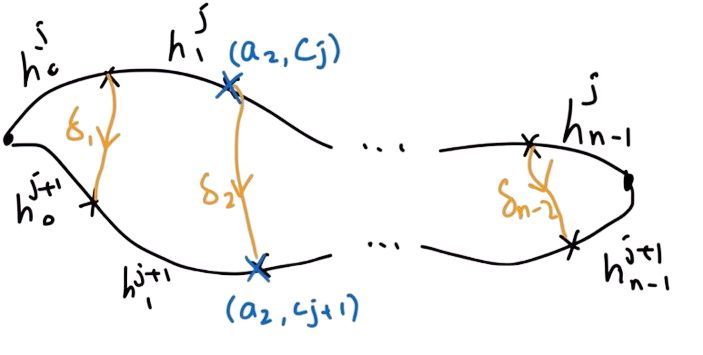
\includegraphics[scale = 0.3]{Image 1}
\end{center}

Now we have that 
\begin{align*}
u([h^j])&=u([h_{n-1}^j])\circ\cdots\circ u([h_0^j])\\
&=u([h_{n-1}^{j+1}\circ\delta_{n-2}])\circ u([\overline{\delta_{n-2}}\circ h_{n-2}^{j+1}\circ\delta_{n-3}])\circ\cdots\circ u([\overline{\delta_1}\circ h_0^{j+1}])\\
&=u([h_{n-1}^{j+1}])\circ\cdots\circ u([h_0^{j+1}])\\
&=u([h^{j+1}])
\end{align*}
By induction, we conclude that $$u([\alpha])=u([h^0])=u([h^1])=\dots=u([h^k])=u([\beta])$$~\\

Now suppose that $A\subseteq X$. By the above lemma, it is sufficient to show that the square for $A$ is a retract of the square for $X$. Let $x\in U\cap V$ and $a_x\in A\cap U\cap V$ lying in the same path component as $x$. Choose a path $\alpha_x:I\to X$ from $a_x$ to $x$ with $\alpha_x$ being constant if $x\in A$. Do a similar choice for $x\in U\setminus(U\cap V)$ and $x\in V\setminus(U\cap V)$. Define $p_{U\cap V}:\Pi_1(U\cap V)\to\Pi_1(U\cap V)[U\cap V\cap A]$ defined by $x\mapsto a_x$ on objects and $$[x\overset{\alpha}{\to} y]\mapsto\left(a_x\overset{[\alpha_x]}{\to}x\overset{[\alpha]}{\to}y\overset{[\alpha_y]}{\to}a_y\right)$$ and similarly for $p_U$ and $p_V$. This defines the natural transformation $p$ in lemma 5.3.4. We conclude by lemma 5.3.4. 
\end{proof}
\end{thm}

Take $A=\{x_0\}$ be a single point in $U\cap V$. Then this theorem shows that there is a pushout diagram \\~\\
\adjustbox{scale=1.0,center}{\begin{tikzcd}
	{\pi_1(U\cap V,x_0)} & {\pi_1(U,x_0)} \\
	{\pi_1(V,x_0)} & {\pi_1(X,x_0)}
	\arrow[from=1-1, to=1-2]
	\arrow[from=1-1, to=2-1]
	\arrow[from=1-2, to=2-2]
	\arrow[from=2-1, to=2-2]
\end{tikzcd}}\\~\\
in $\bold{Grp}$, provided that $A$ contains every path connected component of $U,V,X$. But $A$ is just one point so the condition becomes that $U,V,X$ and $U\cap V$ being path connected. Hence we recover the usual Seifert-Van Kampen theorem in Algebraic Topology 1. 

\pagebreak
\section{Homology and Cohomology Theories}
We have seen that the homotopy groups, the homology groups and the cohomology groups all satisfy a functorial property. This means that they can be considered as functors from the category of spaces to the category of some algebraic structures. It is meaningful to study all of them at once, and to compare different versions of homology and cohomology. \\~\\

In this section, we will introduce generalized (relative) versions, reduced versions, pointed versions and the ordinary version. 

\subsection{Generalized Homology Theories}
\begin{defn}{Generalized Homology Theory for CW Pairs}{} A Generalized Homology Theory is a collection of functors and natural transformations $$h_n:\bold{CW}^2\to\bold{Ab}\;\;\;\;\;\;\;\text{ and }\;\;\;\;\;\;\;\delta_n:h_n(X,Y)\to h_{n-1}(Y,\emptyset)$$ satisfying the following. 
\begin{itemize}
\item Homotopy Invariance: If $f\simeq g:(X,A)\to(Y,B)$ then $$h_n(f)=h_n(g):h_n(X,A)\to h_n(Y,B)$$
\item Exactness: There exists a short exact sequence \\~\\
\adjustbox{scale=0.98,center}{\begin{tikzcd}
	\cdots & {h_{n+1}(X,A)} & {h_n(A,\emptyset)} & {h_n(X,\emptyset)} & {h_n(X,A)} & {h_{n-1}(A,\emptyset)} & \cdots
	\arrow[from=1-1, to=1-2]
	\arrow["{\delta_{n+1}}", from=1-2, to=1-3]
	\arrow["h_n(i)", from=1-3, to=1-4]
	\arrow["h_n(j)", from=1-4, to=1-5]
	\arrow["{\delta_n}", from=1-5, to=1-6]
	\arrow[from=1-6, to=1-7]
\end{tikzcd}}\\~\\
where $i:A\to X$ and $j:X\to(X,A)$ are inclusions. 
\item Additivity: If $(X,A)=\coprod_{i\in I}(X_i,A_i)$, then the direct sum of the inclusion maps $$\bigoplus_{i\in I}h_n(X_i,A_i)\cong h_n(X,A)$$ is an isomorphism
\item Excision: If $\overline{E}\subseteq A^\circ\subseteq X$, then $$h_n(X\setminus E,A\setminus E)\cong h_n(X,A)$$ induced by the inclusion map
\end{itemize}
\end{defn}

We mention for once and for all that the additivity axiom is required only when the CW complexes are finite. In particular, in order for the homology theory to be meaningful, we must restrict the underlying category of spaces to be finite CW complexes if one drops the additivity axiom. 

\begin{lmm}{}{} The excision axiom is equivalent to saying that $X=A^\circ\cup B^\circ$ with inclusion map $\iota:(B,A\cap B)\to (X,A)$ implies $h_n(\iota):h_n(B,A\cap B)\to h_n(X,A)$ is an isomorphism. 
\end{lmm}

\begin{defn}{Generalized Homology Theory}{} A Generalized Homology Theory is a collection of functors $$h_n:\bold{Top}^2\to\bold{Ab}\;\;\;\;\;\;\;\text{ and }\;\;\;\;\;\;\;\delta_n:h_n(X,Y)\to h_{n-1}(Y,\emptyset)$$ satisfying the firs four axioms together with the following. 
\begin{itemize}
\item Weak Equivalence: If $f:(X,A)\to(Y,B)$ is a weak equivalence, then $$f_\ast:h_n(X,A)\to h_n(Y,B)$$ is an isomorphism. 
\end{itemize}
\end{defn}

By adding on the axiom of weak equivalence and the fact that every space admits a weak equivalence to a CW complex, we can see that the two theories are the same. However, note that in this case some of the working homology theories are not a generalized homology theory in this sense (when we encounter the dual notion, sheaf cohomology is not a generalized cohomology theory). 

\begin{thm}{}{} Any generalized homology theory on $\bold{Top}^2$ determines and is determined by a generalized homology theory on $\bold{CW}^2$.
\end{thm}

\begin{defn}{Ordinary Homology Theory}{} Let $G$ be an abelian group. If a generalized homology theory $(h_n,\delta_n)$ in addition satisfies 
\begin{itemize}
\item Dimension: $$h_n(\ast)=\begin{cases}
G & \text{ if } n=0\\
0 & \text{ otherwise }
\end{cases}$$
\end{itemize}
Then $h_n$ is called an ordinary homology theory. 
\end{defn}

\begin{thm}{Eilenberg-Steenrod Uniqueness Theorem}{} Let $T:(h_n,\delta_n)\to(h_n',\delta_n')$ be a natural transformation of generalized homology theories defined on $\bold{CW}^2$ such that $h_n(\ast)\cong h_n'(\ast)$, then $T$ is a natural isomorphism $$(h_n,\delta_n)\cong(h_n',\delta_n')$$
\end{thm}

\subsection{Reduced Homology Theory}
\begin{defn}{Reduced Homology Theory}{} A reduced Homology Theory is a collection of functors and natural transformations $$\widetilde{h}_n:\bold{CW}\to\bold{Ab}\;\;\;\;\;\;\;\text{ and }\;\;\;\;\;\;\;\delta_n:\widetilde{h}_n(X/A)\to\widetilde{h}_{n-1}(A)$$ satisfying the following. 
\begin{itemize}
\item Homotopy Invariance: If $f\simeq g:X\to Y$ then $$\widetilde{h}_n(f)=\widetilde{h}_n(g):\widetilde{h}_n(X)\to\widetilde{h}_n(Y)$$
\item Exactness: If $X$ is a CW-complex and $A\subseteq X$, then there is a short exact sequence \\~\\
\adjustbox{scale=1.0,center}{\begin{tikzcd}
	\cdots & {\widetilde{h}_{n+1}(X/A)} & {\widetilde{h}_n(A)} & {\widetilde{h}_n(X)} & {\widetilde{h}_n(X/A)} & {\widetilde{h}_{n-1}(A)} & \cdots
	\arrow[from=1-1, to=1-2]
	\arrow["{\delta_{n+1}}", from=1-2, to=1-3]
	\arrow["\widetilde{h}_n(\iota)", from=1-3, to=1-4]
	\arrow["\widetilde{h}_n(\pi)", from=1-4, to=1-5]
	\arrow["{\delta_n}", from=1-5, to=1-6]
	\arrow[from=1-6, to=1-7]
\end{tikzcd}}\\~\\
where $\iota:A\to X$ is the inclusion and $\pi:X\to X/A$ is the projection. 
\item Additivity: If $X=\coprod_{i\in I}X_i$, then the direct sum of the inclusion maps $$\bigoplus_{i\in I}\widetilde{h}_n(X_i)\cong\widetilde{h}_n(X)$$ is an isomorphism
\end{itemize}
\end{defn}

\begin{lmm}{}{} Let $\widetilde{h}_n:\bold{CW}\to\bold{Ab}$ be a reduced homology theory. Then $$\widetilde{h}_n(\ast)=0$$
\end{lmm}

\begin{prp}{}{} Let $\widetilde{h}_n:\bold{CW}\to\bold{Ab}$ be a reduced homology theory. Then there is a natural isomorphism $$\widetilde{h}_{n+1}(\Sigma X)=\widetilde{h}_n(X)$$
\end{prp}

\begin{thm}{}{} Any generalized homology theory determines and is determined by a reduced homology theory.
\end{thm}

\subsection{Cohomology Theories}
\begin{defn}{Generalized Cohomology Theory for CW Pairs}{} A Generalized cohomology theory is a collection of contravariant functors $$h^n:\bold{CW}_2\to\bold{Ab}\;\;\;\;\;\;\;\text{ and }\;\;\;\;\;\;\;\delta^n:h^n(A,\emptyset)\to h^{n+1}(X,A)$$ satisfying the following. 
\begin{itemize}
\item Homotopy Invariance: If $f\simeq g:(X,A)\to(Y,B)$ then $$h^n(f)=h^n(g):h^n(X,A)\to h^n(Y,B)$$
\item Exactness: If $X$ is a CW-complex and $A\subseteq X$, then there is a short exact sequence \\~\\
\adjustbox{scale=1.0,center}{\begin{tikzcd}
	\cdots & {h^n(X/A)} & {h^n(X)} & {h^n(A)} & {h^{n+1}(X/A)} & {h^{n+1}(X)} & \cdots
	\arrow[from=1-1, to=1-2]
	\arrow[from=1-2, to=1-3]
	\arrow[from=1-3, to=1-4]
	\arrow["{\partial_n}", from=1-4, to=1-5]
	\arrow[from=1-5, to=1-6]
	\arrow[from=1-6, to=1-7]
\end{tikzcd}}\\~\\
\item Additivity: If $(X,A)=\coprod_{i\in I}(X_i,A_i)$, then the direct sum of the inclusion maps $$\bigoplus_{i\in I}h^n(X_i,A_i)\cong h^n(X,A)$$ is an isomorphism
\item Excision: If $\overline{E}\subseteq A^\circ\subseteq X$, then $$h^n(X\setminus E,A\setminus E)\cong h^n(X,A)$$ induced by the inclusion map
\end{itemize}
\end{defn}

\begin{defn}{Generalized Cohomology Theory}{} A Generalized cohomology theory is a collection of contravariant functors $$h^n:\bold{Top}_2\to\bold{Ab}\;\;\;\;\;\;\;\text{ and }\;\;\;\;\;\;\;\delta^n:h^n(A,\emptyset)\to h^{n+1}(X,A)$$ satisfying the above first four axioms and the following. 
\begin{itemize}
\item Weak Equivalence: If $f:(X,A)\to(Y,B)$ is a weak equivalence, then $$f_\ast:h^n(Y,B)\to h^n(X,A)$$ is an isomorphism. 
\end{itemize}
\end{defn}

\begin{defn}{Reduced Cohomology Theory for CW Pairs}{} A reduced cohomology theory is a collection of contravariant functors $$\widetilde{h}^n:\bold{CW}\to\bold{Ab}\;\;\;\;\;\;\;\text{ and }\;\;\;\;\;\;\;\delta^n:\widetilde{h}^n(A,\emptyset)\to\widetilde{h}^{n+1}(X,A)$$ satisfying the following. 
\begin{itemize}
\item Homotopy Invariance: If $f\simeq g:X\to Y$ then $$\widetilde{h}^n(f)=\widetilde{h}^n(g):\widetilde{h}^n(X)\to\widetilde{h}^n(Y)$$
\item Exactness: There exists a short exact sequence \\~\\
\adjustbox{scale=1.0,center}{\begin{tikzcd}
	\cdots & {\widetilde{h}^n(X,A)} & {\widetilde{h}^n(X)} & {\widetilde{h}^n(A)} & {\widetilde{h}^{n+1}(X,A)} & {\widetilde{h}^{n+1}(X)} & \cdots
	\arrow[from=1-1, to=1-2]
	\arrow["\widetilde{h}_n(\pi)", from=1-2, to=1-3]
	\arrow["\widetilde{h}_n(\iota)", from=1-3, to=1-4]
	\arrow["{\delta_n}", from=1-4, to=1-5]
	\arrow["\widetilde{h}_{n+1}(\pi)", from=1-5, to=1-6]
	\arrow[from=1-6, to=1-7]
\end{tikzcd}}\\~\\
where $\iota:A\to X$ is the inclusion and $\pi:X\to X/A$ is the projection. 
\item Additivity: If $X=\coprod_{i\in I}X_i$, then the direct sum of the inclusion maps $$\bigoplus_{i\in I}\widetilde{h}^n(X_i)\cong\widetilde{h}^n(X)$$ is an isomorphism
\end{itemize}
\end{defn}

\begin{lmm}{}{} Let $\widetilde{h}_n:\bold{CW}\to\bold{Ab}$ be a reduced homology theory. Then $$\widetilde{h}_n(\ast)=0$$
\end{lmm}

\begin{prp}{}{} Let $\widetilde{h}^n:\bold{CW}\to\bold{Ab}$ be a reduced cohomology theory. Then there is a natural isomorphism $$\widetilde{h}_{n+1}(\Sigma X)=\widetilde{h}_n(X)$$
\end{prp}

TBA: Unreduced = reduced. 










\end{document}
